Saved calibration results let us separate three questions that are often
conflated: does the \textbf{model form} matter, does the \textbf{update
policy} matter, and how much of the answer depends on \textbf{which rows
survive the eligibility filter}? On the 3,493 eligible scored cases
recorded between 2004-11 and 2005-04, model form dominates by a wide
margin. A quadratic specification fitted once and then frozen attains an
RMSE of 0.146, against 2.526 for a frozen linear specification and 1.701
for a monthly-updated linear one. Refitting monthly coincides with lower
error \emph{within} a given form --- pooled RMSE falls by roughly a
third --- but it does not close the gap between forms. The conclusion
these files support is therefore conditional: monthly updating is worth
doing if the deployed form is already adequate, and its recorded compute
cost is negligible within the measured scope; choosing the form is the
far larger decision.

Two scope notes matter for reading everything below. First, all numbers
are computed from the saved result files and their reference tables; no
model was refitted and no new experiment was run for this note. Second,
the saved files name a calibration exercise with a linear and a
quadratic specification but do not record the application domain, the
units or valid range of the target, or any admissibility rule for
negative predicted values. We therefore report quantities as recorded
and avoid physical interpretation; negative predicted values are
counted, not judged.

\hypertarget{what-the-saved-results-cover}{%
\section{What the saved results
cover}\label{what-the-saved-results-cover}}

The evaluation window contains 3,711 scored rows, of which 3,493 pass
the eligibility filter (94.1\%). The 218 excluded rows are concentrated
in three of the six months: December (80 of 744), January (61 of 744)
and February (76 of 672), with essentially none in November, March and
April. November, March and April therefore contribute near-complete
monthly samples, whereas the three winter months contribute
88.7--91.8\%. April is a partial month: the test file ends on 4 April,
so that cohort holds only 87 rows, 2.5\% of the test set, and any
monthly statistic for it is correspondingly imprecise.

The fit window expands from 5,498 rows in November to 8,904 rows in
April as each month's data is appended. The frozen baseline is a single
fit on the training-plus-validation window (5,498 rows); the ``updated''
series refits at the start of each month on everything available up to
that point. The first cohort is therefore identical under both policies
by construction: in November the frozen fit and the first refit are the
same model, so the exact zero difference there (Table 2) is a
bookkeeping identity, not evidence that updating fails to help.

\hypertarget{model-form-versus-update-policy}{%
\section{Model form versus update
policy}\label{model-form-versus-update-policy}}

The primary comparison is pooled across all 3,493 eligible cases and is
summarised in Table 1. Read it in two steps. First compare the two
update policies \emph{within} a form: RMSE drops from 2.526 to 1.701 for
the linear specification and from 0.1465 to 0.0926 for the quadratic,
i.e.~by 32.7\% and 36.8\%. Then compare forms at a fixed policy: the
frozen quadratic has 17.2 times lower RMSE than the frozen linear, and
even the monthly-updated linear (1.701) is 11.6 times worse than the
frozen quadratic (0.1465). The form gap is an order of magnitude larger
than the policy gap, which is the central result of this comparison.

Table 1. Pooled accuracy on the 3,493 eligible scored cases (identical
cases for all four series).

\begin{longtable}[]{@{}llrrrrrrr@{}}
\toprule
\begin{minipage}[b]{0.08\columnwidth}\raggedright
Form\strut
\end{minipage} & \begin{minipage}[b]{0.08\columnwidth}\raggedright
Policy\strut
\end{minipage} & \begin{minipage}[b]{0.08\columnwidth}\raggedleft
n\strut
\end{minipage} & \begin{minipage}[b]{0.08\columnwidth}\raggedleft
RMSE\strut
\end{minipage} & \begin{minipage}[b]{0.08\columnwidth}\raggedleft
MAE\strut
\end{minipage} & \begin{minipage}[b]{0.08\columnwidth}\raggedleft
\textbar bias\textbar{}\strut
\end{minipage} & \begin{minipage}[b]{0.08\columnwidth}\raggedleft
P95 \textbar err\textbar{}\strut
\end{minipage} & \begin{minipage}[b]{0.08\columnwidth}\raggedleft
R\^{}2\strut
\end{minipage} & \begin{minipage}[b]{0.08\columnwidth}\raggedleft
Pred. \textless{} 0\strut
\end{minipage}\tabularnewline
\midrule
\endhead
\begin{minipage}[t]{0.08\columnwidth}\raggedright
linear\strut
\end{minipage} & \begin{minipage}[t]{0.08\columnwidth}\raggedright
frozen\strut
\end{minipage} & \begin{minipage}[t]{0.08\columnwidth}\raggedleft
3493\strut
\end{minipage} & \begin{minipage}[t]{0.08\columnwidth}\raggedleft
2.5261\strut
\end{minipage} & \begin{minipage}[t]{0.08\columnwidth}\raggedleft
2.1287\strut
\end{minipage} & \begin{minipage}[t]{0.08\columnwidth}\raggedleft
1.8965\strut
\end{minipage} & \begin{minipage}[t]{0.08\columnwidth}\raggedleft
4.4509\strut
\end{minipage} & \begin{minipage}[t]{0.08\columnwidth}\raggedleft
0.8923\strut
\end{minipage} & \begin{minipage}[t]{0.08\columnwidth}\raggedleft
644 (18.4\%)\strut
\end{minipage}\tabularnewline
\begin{minipage}[t]{0.08\columnwidth}\raggedright
linear\strut
\end{minipage} & \begin{minipage}[t]{0.08\columnwidth}\raggedright
updated\strut
\end{minipage} & \begin{minipage}[t]{0.08\columnwidth}\raggedleft
3493\strut
\end{minipage} & \begin{minipage}[t]{0.08\columnwidth}\raggedleft
1.7010\strut
\end{minipage} & \begin{minipage}[t]{0.08\columnwidth}\raggedleft
1.1461\strut
\end{minipage} & \begin{minipage}[t]{0.08\columnwidth}\raggedleft
0.7675\strut
\end{minipage} & \begin{minipage}[t]{0.08\columnwidth}\raggedleft
3.1826\strut
\end{minipage} & \begin{minipage}[t]{0.08\columnwidth}\raggedleft
0.9511\strut
\end{minipage} & \begin{minipage}[t]{0.08\columnwidth}\raggedleft
391 (11.2\%)\strut
\end{minipage}\tabularnewline
\begin{minipage}[t]{0.08\columnwidth}\raggedright
quadratic\strut
\end{minipage} & \begin{minipage}[t]{0.08\columnwidth}\raggedright
frozen\strut
\end{minipage} & \begin{minipage}[t]{0.08\columnwidth}\raggedleft
3493\strut
\end{minipage} & \begin{minipage}[t]{0.08\columnwidth}\raggedleft
0.1465\strut
\end{minipage} & \begin{minipage}[t]{0.08\columnwidth}\raggedleft
0.1089\strut
\end{minipage} & \begin{minipage}[t]{0.08\columnwidth}\raggedleft
0.0664\strut
\end{minipage} & \begin{minipage}[t]{0.08\columnwidth}\raggedleft
0.3044\strut
\end{minipage} & \begin{minipage}[t]{0.08\columnwidth}\raggedleft
0.9996\strut
\end{minipage} & \begin{minipage}[t]{0.08\columnwidth}\raggedleft
9 (0.3\%)\strut
\end{minipage}\tabularnewline
\begin{minipage}[t]{0.08\columnwidth}\raggedright
quadratic\strut
\end{minipage} & \begin{minipage}[t]{0.08\columnwidth}\raggedright
updated\strut
\end{minipage} & \begin{minipage}[t]{0.08\columnwidth}\raggedleft
3493\strut
\end{minipage} & \begin{minipage}[t]{0.08\columnwidth}\raggedleft
0.0926\strut
\end{minipage} & \begin{minipage}[t]{0.08\columnwidth}\raggedleft
0.0573\strut
\end{minipage} & \begin{minipage}[t]{0.08\columnwidth}\raggedleft
0.0247\strut
\end{minipage} & \begin{minipage}[t]{0.08\columnwidth}\raggedleft
0.1777\strut
\end{minipage} & \begin{minipage}[t]{0.08\columnwidth}\raggedleft
0.9999\strut
\end{minipage} & \begin{minipage}[t]{0.08\columnwidth}\raggedleft
6 (0.2\%)\strut
\end{minipage}\tabularnewline
\bottomrule
\end{longtable}

Within a form, the updated series also has lower MAE (46.2\% for linear,
47.4\% for quadratic) and lower 95th-percentile absolute error (28.5\%
and 41.6\%). It roughly halves the count of negative predicted values
for the linear specification (644 to 391 cases, 18.4\% to 11.2\% of the
scored set); the quadratic's residual count is 6--9 cases. Because the
saved files record no admissibility rule, no post-processing step and no
valid range for the target, these counts are reported as a descriptive
property of the outputs, and any downstream treatment of them is outside
what the files can establish.

The monthly breakdown (Table 2, Figure 1) shows where the pooled
difference comes from and where it does not. Two features are worth
reporting to a collaborator. First, the difference is absent in the
first month by construction, appears only weakly in December (linear
−4.7\%, quadratic +3.2\%), and then becomes large from January onward:
38.3--55.1\% for the linear specification and 45.8--63.1\% for the
quadratic. Second, the largest percentage differences land in February
and March, which have near-complete coverage (88.7\% and 99.9\%) and
596--743 scored cases, so they are not artifacts of tiny samples.
December is the one genuine counter-example: the monthly refit is
followed by a slightly higher RMSE for the better-specified quadratic
while the same policy coincides with a lower RMSE for the linear
specification.

Table 2. RMSE and MAE by month and form, frozen versus monthly-updated.

\begin{longtable}[]{@{}lrlrrrrr@{}}
\toprule
\begin{minipage}[b]{0.10\columnwidth}\raggedright
Month\strut
\end{minipage} & \begin{minipage}[b]{0.10\columnwidth}\raggedleft
n\strut
\end{minipage} & \begin{minipage}[b]{0.10\columnwidth}\raggedright
Form\strut
\end{minipage} & \begin{minipage}[b]{0.10\columnwidth}\raggedleft
RMSE frozen\strut
\end{minipage} & \begin{minipage}[b]{0.10\columnwidth}\raggedleft
RMSE updated\strut
\end{minipage} & \begin{minipage}[b]{0.10\columnwidth}\raggedleft
Δ RMSE\strut
\end{minipage} & \begin{minipage}[b]{0.10\columnwidth}\raggedleft
MAE frozen\strut
\end{minipage} & \begin{minipage}[b]{0.10\columnwidth}\raggedleft
MAE updated\strut
\end{minipage}\tabularnewline
\midrule
\endhead
\begin{minipage}[t]{0.10\columnwidth}\raggedright
2004-11\strut
\end{minipage} & \begin{minipage}[t]{0.10\columnwidth}\raggedleft
720\strut
\end{minipage} & \begin{minipage}[t]{0.10\columnwidth}\raggedright
linear\strut
\end{minipage} & \begin{minipage}[t]{0.10\columnwidth}\raggedleft
1.8974\strut
\end{minipage} & \begin{minipage}[t]{0.10\columnwidth}\raggedleft
1.8974\strut
\end{minipage} & \begin{minipage}[t]{0.10\columnwidth}\raggedleft
0.0\%\strut
\end{minipage} & \begin{minipage}[t]{0.10\columnwidth}\raggedleft
1.3265\strut
\end{minipage} & \begin{minipage}[t]{0.10\columnwidth}\raggedleft
1.3265\strut
\end{minipage}\tabularnewline
\begin{minipage}[t]{0.10\columnwidth}\raggedright
2004-11\strut
\end{minipage} & \begin{minipage}[t]{0.10\columnwidth}\raggedleft
720\strut
\end{minipage} & \begin{minipage}[t]{0.10\columnwidth}\raggedright
quadratic\strut
\end{minipage} & \begin{minipage}[t]{0.10\columnwidth}\raggedleft
0.0989\strut
\end{minipage} & \begin{minipage}[t]{0.10\columnwidth}\raggedleft
0.0989\strut
\end{minipage} & \begin{minipage}[t]{0.10\columnwidth}\raggedleft
0.0\%\strut
\end{minipage} & \begin{minipage}[t]{0.10\columnwidth}\raggedleft
0.0612\strut
\end{minipage} & \begin{minipage}[t]{0.10\columnwidth}\raggedleft
0.0612\strut
\end{minipage}\tabularnewline
\begin{minipage}[t]{0.10\columnwidth}\raggedright
2004-12\strut
\end{minipage} & \begin{minipage}[t]{0.10\columnwidth}\raggedleft
664\strut
\end{minipage} & \begin{minipage}[t]{0.10\columnwidth}\raggedright
linear\strut
\end{minipage} & \begin{minipage}[t]{0.10\columnwidth}\raggedleft
2.3825\strut
\end{minipage} & \begin{minipage}[t]{0.10\columnwidth}\raggedleft
2.2712\strut
\end{minipage} & \begin{minipage}[t]{0.10\columnwidth}\raggedleft
−4.7\%\strut
\end{minipage} & \begin{minipage}[t]{0.10\columnwidth}\raggedleft
1.7290\strut
\end{minipage} & \begin{minipage}[t]{0.10\columnwidth}\raggedleft
1.3802\strut
\end{minipage}\tabularnewline
\begin{minipage}[t]{0.10\columnwidth}\raggedright
2004-12\strut
\end{minipage} & \begin{minipage}[t]{0.10\columnwidth}\raggedleft
664\strut
\end{minipage} & \begin{minipage}[t]{0.10\columnwidth}\raggedright
quadratic\strut
\end{minipage} & \begin{minipage}[t]{0.10\columnwidth}\raggedleft
0.1263\strut
\end{minipage} & \begin{minipage}[t]{0.10\columnwidth}\raggedleft
0.1304\strut
\end{minipage} & \begin{minipage}[t]{0.10\columnwidth}\raggedleft
+3.2\%\strut
\end{minipage} & \begin{minipage}[t]{0.10\columnwidth}\raggedleft
0.0832\strut
\end{minipage} & \begin{minipage}[t]{0.10\columnwidth}\raggedleft
0.0677\strut
\end{minipage}\tabularnewline
\begin{minipage}[t]{0.10\columnwidth}\raggedright
2005-01\strut
\end{minipage} & \begin{minipage}[t]{0.10\columnwidth}\raggedleft
683\strut
\end{minipage} & \begin{minipage}[t]{0.10\columnwidth}\raggedright
linear\strut
\end{minipage} & \begin{minipage}[t]{0.10\columnwidth}\raggedleft
2.4427\strut
\end{minipage} & \begin{minipage}[t]{0.10\columnwidth}\raggedleft
1.5072\strut
\end{minipage} & \begin{minipage}[t]{0.10\columnwidth}\raggedleft
−38.3\%\strut
\end{minipage} & \begin{minipage}[t]{0.10\columnwidth}\raggedleft
2.1872\strut
\end{minipage} & \begin{minipage}[t]{0.10\columnwidth}\raggedleft
1.0556\strut
\end{minipage}\tabularnewline
\begin{minipage}[t]{0.10\columnwidth}\raggedright
2005-01\strut
\end{minipage} & \begin{minipage}[t]{0.10\columnwidth}\raggedleft
683\strut
\end{minipage} & \begin{minipage}[t]{0.10\columnwidth}\raggedright
quadratic\strut
\end{minipage} & \begin{minipage}[t]{0.10\columnwidth}\raggedleft
0.1410\strut
\end{minipage} & \begin{minipage}[t]{0.10\columnwidth}\raggedleft
0.0764\strut
\end{minipage} & \begin{minipage}[t]{0.10\columnwidth}\raggedleft
−45.8\%\strut
\end{minipage} & \begin{minipage}[t]{0.10\columnwidth}\raggedleft
0.1106\strut
\end{minipage} & \begin{minipage}[t]{0.10\columnwidth}\raggedleft
0.0516\strut
\end{minipage}\tabularnewline
\begin{minipage}[t]{0.10\columnwidth}\raggedright
2005-02\strut
\end{minipage} & \begin{minipage}[t]{0.10\columnwidth}\raggedleft
596\strut
\end{minipage} & \begin{minipage}[t]{0.10\columnwidth}\raggedright
linear\strut
\end{minipage} & \begin{minipage}[t]{0.10\columnwidth}\raggedleft
2.8479\strut
\end{minipage} & \begin{minipage}[t]{0.10\columnwidth}\raggedleft
1.2785\strut
\end{minipage} & \begin{minipage}[t]{0.10\columnwidth}\raggedleft
−55.1\%\strut
\end{minipage} & \begin{minipage}[t]{0.10\columnwidth}\raggedleft
2.6518\strut
\end{minipage} & \begin{minipage}[t]{0.10\columnwidth}\raggedleft
0.9211\strut
\end{minipage}\tabularnewline
\begin{minipage}[t]{0.10\columnwidth}\raggedright
2005-02\strut
\end{minipage} & \begin{minipage}[t]{0.10\columnwidth}\raggedleft
596\strut
\end{minipage} & \begin{minipage}[t]{0.10\columnwidth}\raggedright
quadratic\strut
\end{minipage} & \begin{minipage}[t]{0.10\columnwidth}\raggedleft
0.1704\strut
\end{minipage} & \begin{minipage}[t]{0.10\columnwidth}\raggedleft
0.0629\strut
\end{minipage} & \begin{minipage}[t]{0.10\columnwidth}\raggedleft
−63.1\%\strut
\end{minipage} & \begin{minipage}[t]{0.10\columnwidth}\raggedleft
0.1391\strut
\end{minipage} & \begin{minipage}[t]{0.10\columnwidth}\raggedleft
0.0448\strut
\end{minipage}\tabularnewline
\begin{minipage}[t]{0.10\columnwidth}\raggedright
2005-03\strut
\end{minipage} & \begin{minipage}[t]{0.10\columnwidth}\raggedleft
743\strut
\end{minipage} & \begin{minipage}[t]{0.10\columnwidth}\raggedright
linear\strut
\end{minipage} & \begin{minipage}[t]{0.10\columnwidth}\raggedleft
2.7791\strut
\end{minipage} & \begin{minipage}[t]{0.10\columnwidth}\raggedleft
1.3089\strut
\end{minipage} & \begin{minipage}[t]{0.10\columnwidth}\raggedleft
−52.9\%\strut
\end{minipage} & \begin{minipage}[t]{0.10\columnwidth}\raggedleft
2.6044\strut
\end{minipage} & \begin{minipage}[t]{0.10\columnwidth}\raggedleft
0.9736\strut
\end{minipage}\tabularnewline
\begin{minipage}[t]{0.10\columnwidth}\raggedright
2005-03\strut
\end{minipage} & \begin{minipage}[t]{0.10\columnwidth}\raggedleft
743\strut
\end{minipage} & \begin{minipage}[t]{0.10\columnwidth}\raggedright
quadratic\strut
\end{minipage} & \begin{minipage}[t]{0.10\columnwidth}\raggedleft
0.1686\strut
\end{minipage} & \begin{minipage}[t]{0.10\columnwidth}\raggedleft
0.0777\strut
\end{minipage} & \begin{minipage}[t]{0.10\columnwidth}\raggedleft
−53.9\%\strut
\end{minipage} & \begin{minipage}[t]{0.10\columnwidth}\raggedleft
0.1389\strut
\end{minipage} & \begin{minipage}[t]{0.10\columnwidth}\raggedleft
0.0578\strut
\end{minipage}\tabularnewline
\begin{minipage}[t]{0.10\columnwidth}\raggedright
2005-04\strut
\end{minipage} & \begin{minipage}[t]{0.10\columnwidth}\raggedleft
87\strut
\end{minipage} & \begin{minipage}[t]{0.10\columnwidth}\raggedright
linear\strut
\end{minipage} & \begin{minipage}[t]{0.10\columnwidth}\raggedleft
3.8365\strut
\end{minipage} & \begin{minipage}[t]{0.10\columnwidth}\raggedleft
1.8287\strut
\end{minipage} & \begin{minipage}[t]{0.10\columnwidth}\raggedleft
−52.3\%\strut
\end{minipage} & \begin{minipage}[t]{0.10\columnwidth}\raggedleft
3.7127\strut
\end{minipage} & \begin{minipage}[t]{0.10\columnwidth}\raggedleft
1.5915\strut
\end{minipage}\tabularnewline
\begin{minipage}[t]{0.10\columnwidth}\raggedright
2005-04\strut
\end{minipage} & \begin{minipage}[t]{0.10\columnwidth}\raggedleft
87\strut
\end{minipage} & \begin{minipage}[t]{0.10\columnwidth}\raggedright
quadratic\strut
\end{minipage} & \begin{minipage}[t]{0.10\columnwidth}\raggedleft
0.2465\strut
\end{minipage} & \begin{minipage}[t]{0.10\columnwidth}\raggedleft
0.0955\strut
\end{minipage} & \begin{minipage}[t]{0.10\columnwidth}\raggedleft
−61.3\%\strut
\end{minipage} & \begin{minipage}[t]{0.10\columnwidth}\raggedleft
0.2239\strut
\end{minipage} & \begin{minipage}[t]{0.10\columnwidth}\raggedleft
0.0732\strut
\end{minipage}\tabularnewline
\bottomrule
\end{longtable}

\begin{figure}[htbp]
\centering
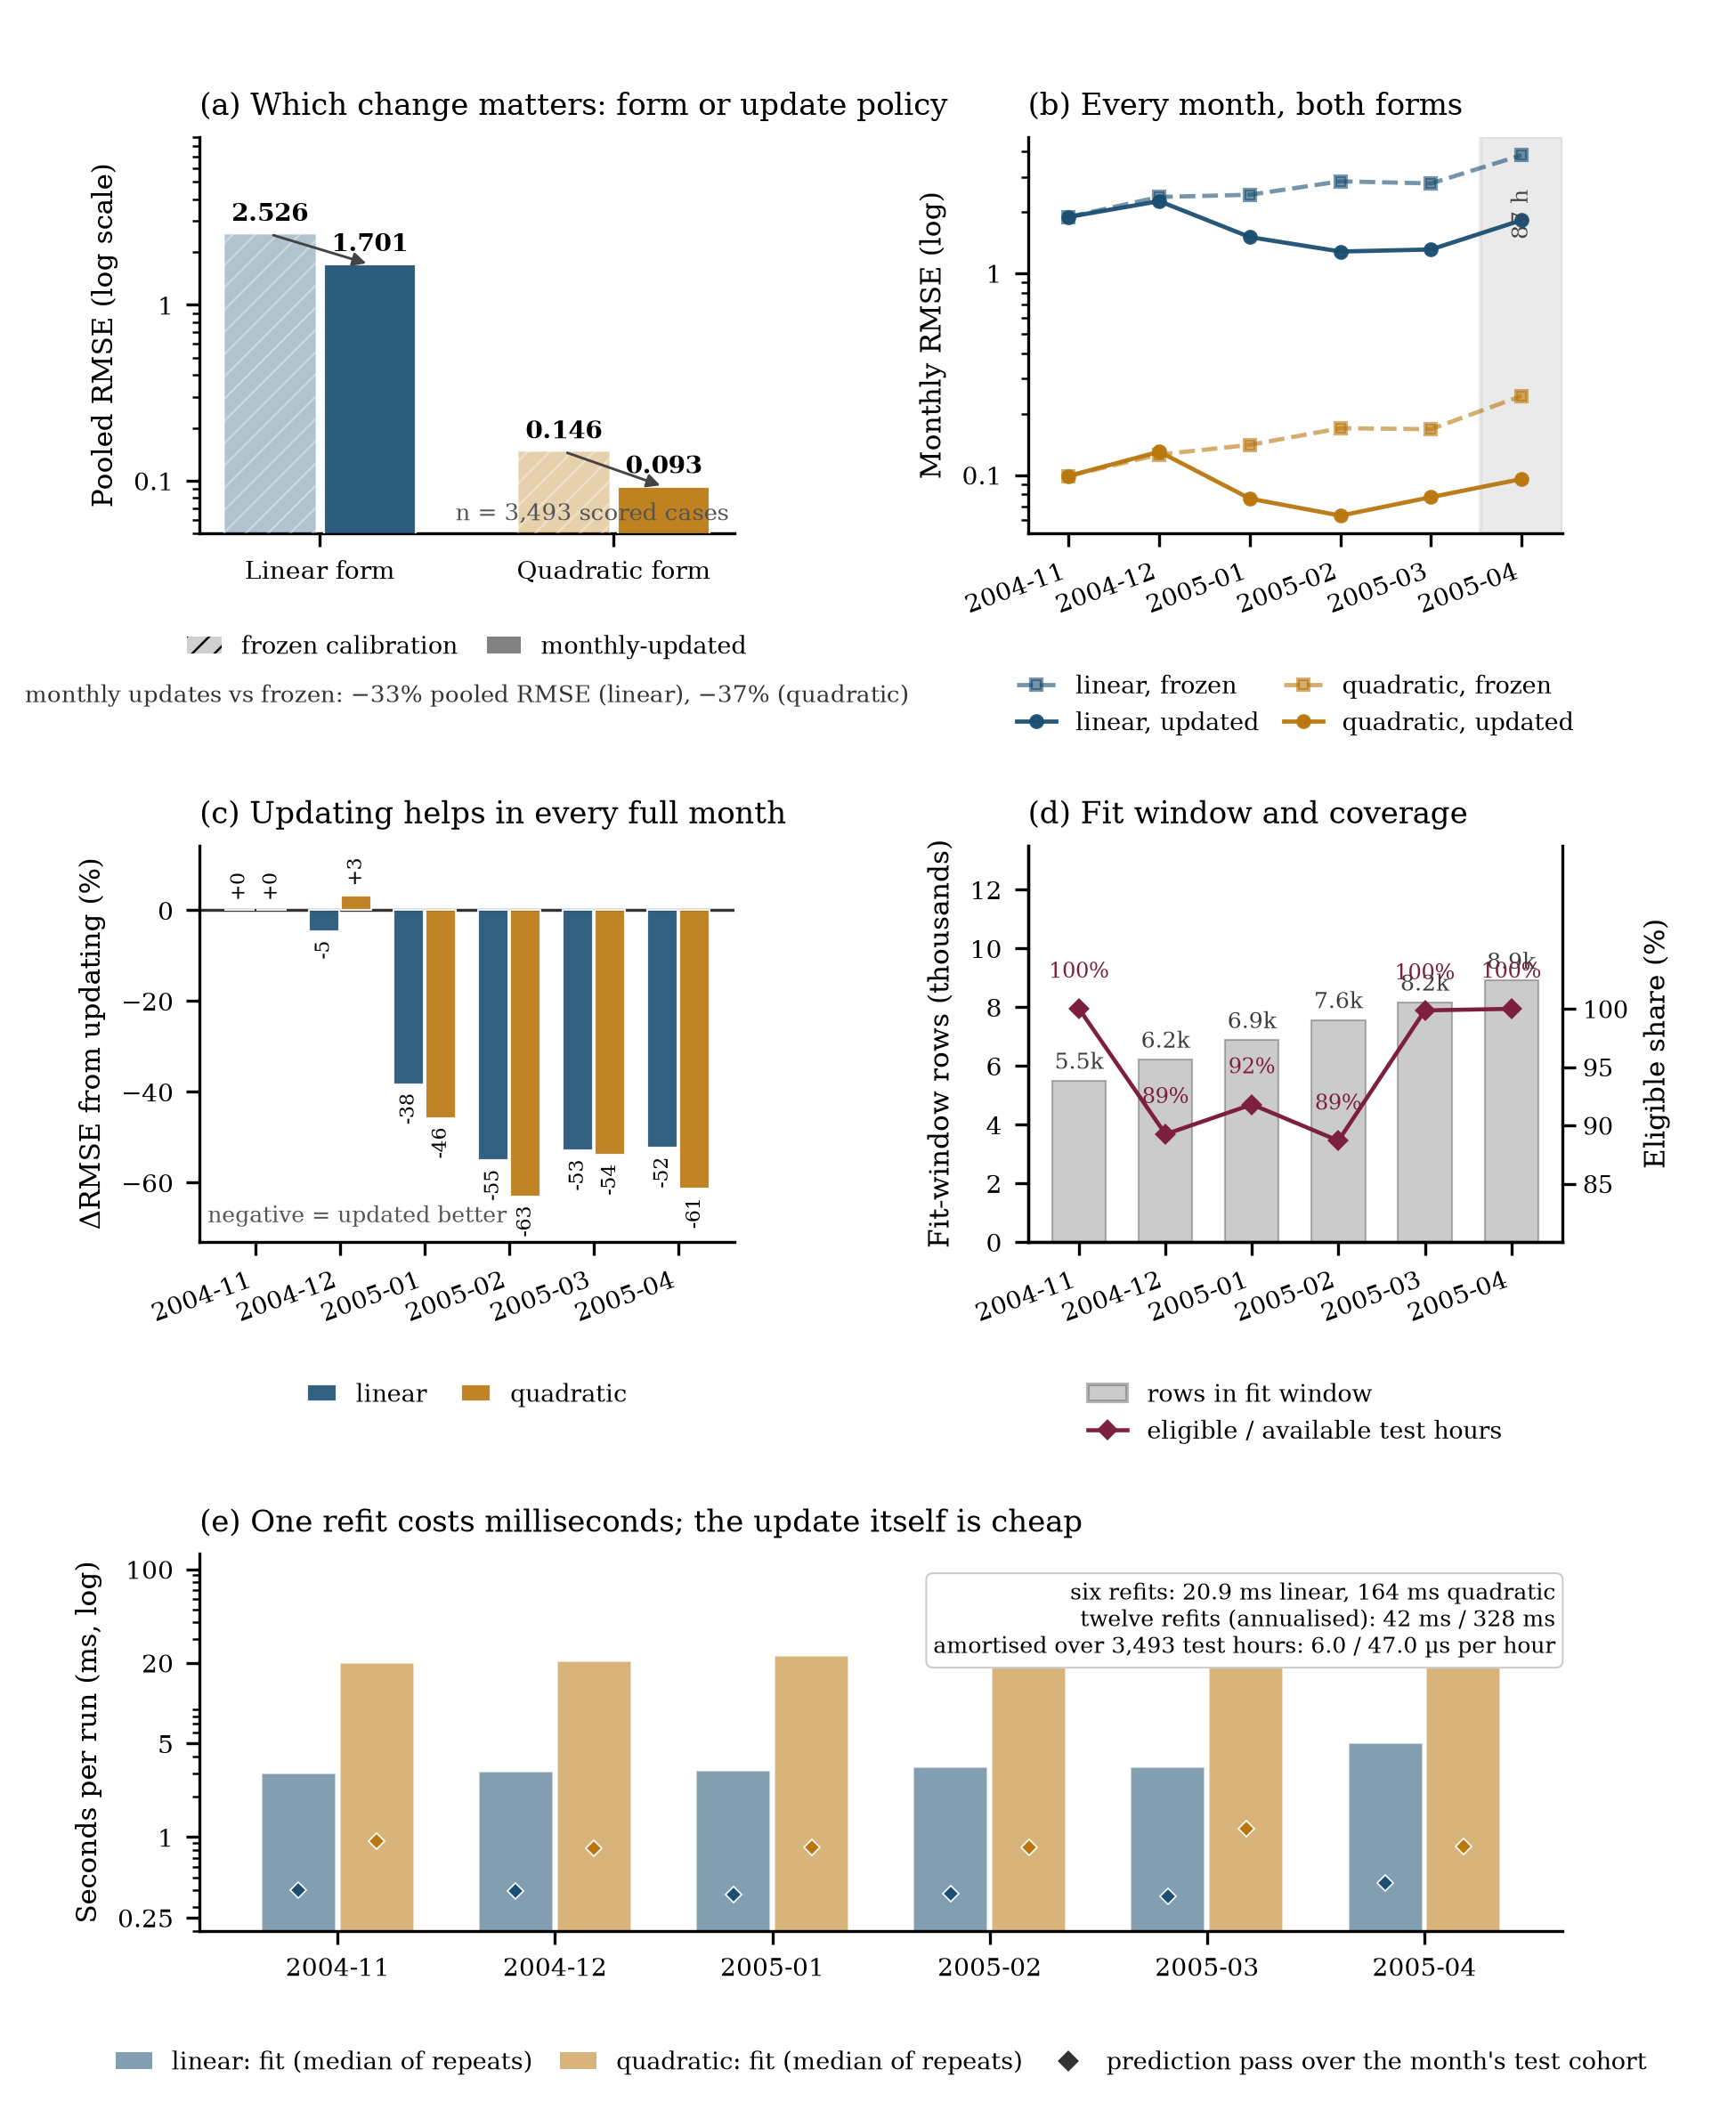
\includegraphics[width=0.84\textwidth,height=\textheight]{figures/figure-1.png}
\caption{Monthly effect of the update policy and its sample coverage.
(a) Pooled RMSE by form and policy on a log scale, with an arrow from
the frozen to the monthly-updated bar for each form and the pooled
percentage change annotated. (b) Monthly RMSE for both forms under both
policies; the partial 2005-04 cohort, shaded, holds only 87 scored
cases. (c) Per-month percentage change in RMSE from updating, separately
for each form; bars below zero mean the updated fit had the lower RMSE,
and 2004-11 is exactly zero because both policies use the same first
fit. (d) Rows in the monthly fit window (bars, left axis) against the
share of available test cases that pass the eligibility filter (line,
right axis). (e) Recorded median fit time (bars) and one prediction pass
(diamonds) per month on a log scale, with six-month sums, annualised
twelve-refit sums and amortised cost annotated. Legends are placed
outside the plotting areas.}
\end{figure}

\hypertarget{sample-coverage}{%
\section{Sample coverage}\label{sample-coverage}}

Coverage is a property of the eligibility filter, not of the model, and
the same 3,493 cases are scored for all four series, so the pooled
comparison is not distorted by different evaluation sets. What coverage
does affect is how much each monthly number can be trusted, and how the
results would transport to a period with a different exclusion rate.

Table 3. Test-case coverage and fit-window size by month.

\begin{longtable}[]{@{}lrrrrrr@{}}
\toprule
\begin{minipage}[b]{0.12\columnwidth}\raggedright
Month\strut
\end{minipage} & \begin{minipage}[b]{0.12\columnwidth}\raggedleft
Fit rows\strut
\end{minipage} & \begin{minipage}[b]{0.12\columnwidth}\raggedleft
Test rows avail.\strut
\end{minipage} & \begin{minipage}[b]{0.12\columnwidth}\raggedleft
Eligible\strut
\end{minipage} & \begin{minipage}[b]{0.12\columnwidth}\raggedleft
Excluded\strut
\end{minipage} & \begin{minipage}[b]{0.12\columnwidth}\raggedleft
Coverage\strut
\end{minipage} & \begin{minipage}[b]{0.12\columnwidth}\raggedleft
Share of test\strut
\end{minipage}\tabularnewline
\midrule
\endhead
\begin{minipage}[t]{0.12\columnwidth}\raggedright
2004-11\strut
\end{minipage} & \begin{minipage}[t]{0.12\columnwidth}\raggedleft
5,498\strut
\end{minipage} & \begin{minipage}[t]{0.12\columnwidth}\raggedleft
720\strut
\end{minipage} & \begin{minipage}[t]{0.12\columnwidth}\raggedleft
720\strut
\end{minipage} & \begin{minipage}[t]{0.12\columnwidth}\raggedleft
0\strut
\end{minipage} & \begin{minipage}[t]{0.12\columnwidth}\raggedleft
100.0\%\strut
\end{minipage} & \begin{minipage}[t]{0.12\columnwidth}\raggedleft
20.6\%\strut
\end{minipage}\tabularnewline
\begin{minipage}[t]{0.12\columnwidth}\raggedright
2004-12\strut
\end{minipage} & \begin{minipage}[t]{0.12\columnwidth}\raggedleft
6,218\strut
\end{minipage} & \begin{minipage}[t]{0.12\columnwidth}\raggedleft
744\strut
\end{minipage} & \begin{minipage}[t]{0.12\columnwidth}\raggedleft
664\strut
\end{minipage} & \begin{minipage}[t]{0.12\columnwidth}\raggedleft
80\strut
\end{minipage} & \begin{minipage}[t]{0.12\columnwidth}\raggedleft
89.2\%\strut
\end{minipage} & \begin{minipage}[t]{0.12\columnwidth}\raggedleft
19.0\%\strut
\end{minipage}\tabularnewline
\begin{minipage}[t]{0.12\columnwidth}\raggedright
2005-01\strut
\end{minipage} & \begin{minipage}[t]{0.12\columnwidth}\raggedleft
6,882\strut
\end{minipage} & \begin{minipage}[t]{0.12\columnwidth}\raggedleft
744\strut
\end{minipage} & \begin{minipage}[t]{0.12\columnwidth}\raggedleft
683\strut
\end{minipage} & \begin{minipage}[t]{0.12\columnwidth}\raggedleft
61\strut
\end{minipage} & \begin{minipage}[t]{0.12\columnwidth}\raggedleft
91.8\%\strut
\end{minipage} & \begin{minipage}[t]{0.12\columnwidth}\raggedleft
19.6\%\strut
\end{minipage}\tabularnewline
\begin{minipage}[t]{0.12\columnwidth}\raggedright
2005-02\strut
\end{minipage} & \begin{minipage}[t]{0.12\columnwidth}\raggedleft
7,565\strut
\end{minipage} & \begin{minipage}[t]{0.12\columnwidth}\raggedleft
672\strut
\end{minipage} & \begin{minipage}[t]{0.12\columnwidth}\raggedleft
596\strut
\end{minipage} & \begin{minipage}[t]{0.12\columnwidth}\raggedleft
76\strut
\end{minipage} & \begin{minipage}[t]{0.12\columnwidth}\raggedleft
88.7\%\strut
\end{minipage} & \begin{minipage}[t]{0.12\columnwidth}\raggedleft
17.1\%\strut
\end{minipage}\tabularnewline
\begin{minipage}[t]{0.12\columnwidth}\raggedright
2005-03\strut
\end{minipage} & \begin{minipage}[t]{0.12\columnwidth}\raggedleft
8,161\strut
\end{minipage} & \begin{minipage}[t]{0.12\columnwidth}\raggedleft
744\strut
\end{minipage} & \begin{minipage}[t]{0.12\columnwidth}\raggedleft
743\strut
\end{minipage} & \begin{minipage}[t]{0.12\columnwidth}\raggedleft
1\strut
\end{minipage} & \begin{minipage}[t]{0.12\columnwidth}\raggedleft
99.9\%\strut
\end{minipage} & \begin{minipage}[t]{0.12\columnwidth}\raggedleft
21.3\%\strut
\end{minipage}\tabularnewline
\begin{minipage}[t]{0.12\columnwidth}\raggedright
2005-04\strut
\end{minipage} & \begin{minipage}[t]{0.12\columnwidth}\raggedleft
8,904\strut
\end{minipage} & \begin{minipage}[t]{0.12\columnwidth}\raggedleft
87\strut
\end{minipage} & \begin{minipage}[t]{0.12\columnwidth}\raggedleft
87\strut
\end{minipage} & \begin{minipage}[t]{0.12\columnwidth}\raggedleft
0\strut
\end{minipage} & \begin{minipage}[t]{0.12\columnwidth}\raggedleft
100.0\%\strut
\end{minipage} & \begin{minipage}[t]{0.12\columnwidth}\raggedleft
2.5\%\strut
\end{minipage}\tabularnewline
\begin{minipage}[t]{0.12\columnwidth}\raggedright
test total\strut
\end{minipage} & \begin{minipage}[t]{0.12\columnwidth}\raggedleft
---\strut
\end{minipage} & \begin{minipage}[t]{0.12\columnwidth}\raggedleft
3,711\strut
\end{minipage} & \begin{minipage}[t]{0.12\columnwidth}\raggedleft
3,493\strut
\end{minipage} & \begin{minipage}[t]{0.12\columnwidth}\raggedleft
218\strut
\end{minipage} & \begin{minipage}[t]{0.12\columnwidth}\raggedleft
94.1\%\strut
\end{minipage} & \begin{minipage}[t]{0.12\columnwidth}\raggedleft
100.0\%\strut
\end{minipage}\tabularnewline
\bottomrule
\end{longtable}

The excluded rows are not analysed here: the saved results record how
many were dropped but not how the models would have performed on them.
Since the dropped rows are the ones the filter judged unusable, the
reported errors are best read as performance on eligible cases. If the
exclusion rule removes exactly the hard cases, the operational error
would be higher than 0.093 (quadratic, updated); the saved files cannot
settle this either way.

\hypertarget{cost-of-updating}{%
\section{Cost of updating}\label{cost-of-updating}}

The recorded timings are medians of repeated in-process measurements,
and they are small (Table 4). A linear refit takes 3.0--5.0 ms, a
quadratic refit 19.8--39.6 ms; a prediction pass over one month's cohort
takes 0.36--0.46 ms and 0.83--1.15 ms respectively. Six refits in total
cost 20.9 ms (linear) and 164.0 ms (quadratic). Three different
normalisations are easy to confuse, so the table keeps them in separate
columns: per-month medians, sums of those six medians, and an annualised
scenario of twelve refits. Dividing the six-month measured totals by the
3,493 scored cases gives about 6.0 µs and 47.0 µs per case, whereas
annualising the refit cost to twelve refits (41.8 ms and 328.0 ms) and
dividing by the same cases gives about 12.0 µs and 93.9 µs. The
six-month figures are \emph{not} annualised costs, and the totals are
sums of the six monthly medians, not per-row costs.

Table 4. Recorded refit and prediction time: monthly medians, their
six-month sums, and a separate annualised scenario.

\begin{longtable}[]{@{}lrrrrr@{}}
\toprule
\begin{minipage}[b]{0.11\columnwidth}\raggedright
Form\strut
\end{minipage} & \begin{minipage}[b]{0.14\columnwidth}\raggedleft
Six refits (ms)\strut
\end{minipage} & \begin{minipage}[b]{0.14\columnwidth}\raggedleft
Six predict passes (ms)\strut
\end{minipage} & \begin{minipage}[b]{0.14\columnwidth}\raggedleft
Annualised refits (ms)\strut
\end{minipage} & \begin{minipage}[b]{0.14\columnwidth}\raggedleft
\seqsplit{{µ}s/scored} case, six-month basis\strut
\end{minipage} & \begin{minipage}[b]{0.14\columnwidth}\raggedleft
\seqsplit{{µ}s/scored} case, annualised basis\strut
\end{minipage}\tabularnewline
\midrule
\endhead
\begin{minipage}[t]{0.11\columnwidth}\raggedright
linear\strut
\end{minipage} & \begin{minipage}[t]{0.14\columnwidth}\raggedleft
20.88\strut
\end{minipage} & \begin{minipage}[t]{0.14\columnwidth}\raggedleft
2.37\strut
\end{minipage} & \begin{minipage}[t]{0.14\columnwidth}\raggedleft
41.8\strut
\end{minipage} & \begin{minipage}[t]{0.14\columnwidth}\raggedleft
6.0\strut
\end{minipage} & \begin{minipage}[t]{0.14\columnwidth}\raggedleft
12.0\strut
\end{minipage}\tabularnewline
\begin{minipage}[t]{0.11\columnwidth}\raggedright
quadratic\strut
\end{minipage} & \begin{minipage}[t]{0.14\columnwidth}\raggedleft
164.02\strut
\end{minipage} & \begin{minipage}[t]{0.14\columnwidth}\raggedleft
5.43\strut
\end{minipage} & \begin{minipage}[t]{0.14\columnwidth}\raggedleft
328.0\strut
\end{minipage} & \begin{minipage}[t]{0.14\columnwidth}\raggedleft
47.0\strut
\end{minipage} & \begin{minipage}[t]{0.14\columnwidth}\raggedleft
93.9\strut
\end{minipage}\tabularnewline
\bottomrule
\end{longtable}

The per-row figures recorded per month are 0.49--0.64 µs (linear) and
1.23--1.54 µs (quadratic) for the five full months, but 5.23 and 9.78 µs
for April. Dividing the recorded prediction time by the batch size
reproduces the eligible-case counts exactly, so the April spike is fixed
per-call overhead spread over an 87-row batch, not a real increase in
marginal cost. Reporting the April figure as ``the'' per-row cost would
overstate prediction cost by roughly an order of magnitude.

These numbers cover only the fit and predict calls. Data ingestion,
feature construction, evaluation and plotting are outside the recorded
scope, and on a real system they plausibly dominate. The defensible
claim is narrow: \emph{within the recorded scope}, a monthly refit is
negligible (0.04 s and 0.33 s of refit compute per year under the
annualised scenario), so recorded compute is not a reason to prefer a
frozen model. It is not evidence about the total cost of running a
monthly pipeline in deployment.

\hypertarget{what-this-does-and-does-not-establish}{%
\section{What this does and does not
establish}\label{what-this-does-and-does-not-establish}}

Supported by the saved results: on the 3,493 eligible cases, model form
dominates update policy; within each form, the monthly-updated series
has roughly a third lower RMSE and about half lower MAE; the difference
grows as the fit window lengthens and is absent by construction in the
first month; coverage varies from 88.7\% to 100\% by month; recorded fit
and prediction times are on the order of milliseconds; and the pooled
metrics are reproducible from the monthly rows (the accompanying script
re-derives pooled RMSE, MAE and bias from Table 2 to within 1e-9).

Not established: whether a monthly schedule would still help under a
\emph{different} form or after hyperparameter retuning --- no retuning
was run, so ``quadratic'' here means the specific saved specification,
and nothing in these results shows how a retuned linear model would
behave (a 17-fold gap makes full closure unlikely, but that is an
extrapolation, not a measurement). Nor is anything established about
models with dependence structure across rows, about performance on the
218 excluded rows, about periods outside 2004-11 to 2005-04, or about
deployment cost including data engineering. The comparison is
descriptive: the two policies differ in fit window and in the data each
sees, so the recorded differences are associations in these files, not
an isolated causal effect of ``updating''. No uncertainty intervals were
computed: the monthly percentages are point estimates on 87--743 cases,
and April in particular should be read as indicative only. Timing values
come from one machine and one process, and the last cohort's per-row
cost is a small-batch artifact.

\hypertarget{recommendation}{%
\section{Recommendation}\label{recommendation}}

Treat the two decisions separately. First choose the form, using pooled
RMSE, MAE, tail error and the count of negative predictions; on this
evidence the quadratic specification is the one worth operating. Then,
given that form, refit monthly: the error difference is consistent from
January onward, refit compute is a fraction of a second per year within
the measured scope, and the only counter-example is December, early in
the window when the fit history is shortest. Keep the frozen benchmark
in reporting so the update's contribution stays visible, and report
coverage alongside accuracy so readers can see which cases the
comparison actually covers. If the form is later retuned or replaced,
the monthly-updating question should be re-answered from new evidence
rather than carried over from this note.
